\documentclass[11pt]{article}
\usepackage{graphicx}
\usepackage{fullpage}
\usepackage{fourier}
\usepackage{xspace}
\usepackage{booktabs}
\usepackage{wrapfig}

\title{cse13s asgn7 WRITEUP.pdf}
\author{Lucas Lee; CruzID: luclee}
\date{3/11/2022}
\begin{document}\maketitle

\section{Program Details}\label{ss:details}
This program will use Hash tables, Bloom Filters, and Bitvectors to find k most likely authors to a given text. 

\section{Program issues, Hash table/Bloom filters}\label{ss:issues}
My program produces the same order of authors as the example binary when I run the program with the normal database, but it runs very slowly compared to the example. This is because my program uses an insertion method rather than the heap method which makes my program run at O(n). Other than this, my program's excessively long run time could be because I may be performing extra hash table lookups throughout the process of computing the distances between the texts and/or computing the Texts. \\
\\
In terms of the smaller databases, the program still runs a bit slow, but the difference is much less than the example binary. For the large databases, it takes about 3 minutes and a half, while running it on the small database is about 20 seconds to run. The accuracy on smaller text files is a bit off, but the order is generally correct with the larger database. There are some files in the small database that sometimes display the wrong ordering, but the only thing that it changes is that it swaps two different texts. The distances for these texts may have something to do with my lookup function, as when I would change the function for testing purposes, it would change the distance to be closer between those two texts. I believe this is when you run the small database to display 10 matches, and the two swapped authors are Henry James and H. G. Wells. Otherwise I have not seen any differences with the result ordering for my program and the example binary.
\\ \\
In the specifics of this program, we had to use bloom filters alongside the hash tables, and what made this program run much slower was the linear probing that we had to implement inside of our hash tables to look for specific words. 
Since we are hashing the words somewhat randomly throughout the hash table that has \(2^{19}\) indices, if a text is larger, then the linear probing will take a long time. The large hash table allows for us to avoid as many hash collisions as possible, which makes the linear probing process happen less frequently, speeding up the process as well. The bloom filter only speeds up the process of lookups in the event that a word is not inside of the hash table, otherwise it has to perform another hash table lookup, which makes the program run longer. In larger texts, this is going to make the process much slower, since many more bits at being set in the bloom filter for each word, there is a higher probability for false positives since the bit vector will be more full of set bits. This could also be why the program's run time is extremely long for the larger databases.

\section{Results when changing noise words}\label{ss:noise}
When changing the noise limit, the speed at which the identify binary changes, as well as many of the results.\\
If you increase the noise limit to around 200, meaning you filter out double the amount of words, the program runs a bit faster than it did before but not by a large difference. In the small database it makes it run a fraction of a second faster because it does not have to check the texts for as many words. For the default database, it decreases the run time by a couple seconds due to the text having much less words since there are much more texts to be created. 
\\ \\
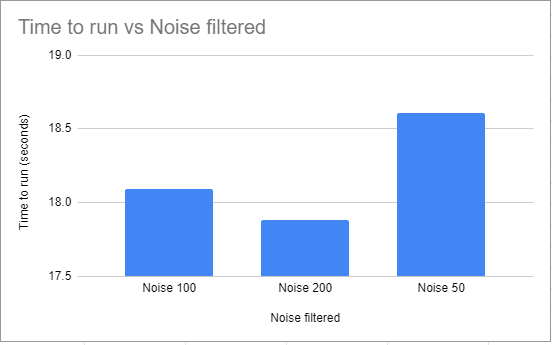
\includegraphics[width = 0.75\textwidth]{Graphs/Noise.PNG}
\\ \\
If you decrease the noise limit to about 50, you are leaving in half as many words that would normally be filtered out, making the program run slower. For the smaller database, this does not matter as much, most likely because the texts in the smaller database use the 50 words, that are not filtering out, very rarely. The run time changes for the small database by about half a second, while for the larger database, it runs for about an extra 15 seconds.
\\ \\
This does not just affect the run time, however. Because increasing noise limit reduces more words in each text, this will also change the words in each text, depending on if those texts contain the extra words we are cutting out. This could also change the ordering of the authors, since some authors' texts could contain more noise words than another. The difference in distance varies with each author because of this, leading to a change in the top k authors, depending on how much the noise affects the texts. This noise change does not affect the top author only if the given text through stdin is an author whose text exists inside the database, because the distance for that author will be 0 regardless, so changing noise text will not change the identification of the correct author.
\\ \\
\section{Comparing large vs small texts}\label{ss:size}
My program correctly is able to identify the closest authors using small texts. For extremely large texts, the amount of words is so large that the numbers calculated for the distances are very close. The distance values are sometimes extremely close when comparing two different large texts because of the amount of words in those texts. In a large text, the text creation process will take much longer because of the hash tables and bloom filters for those texts. In the Program issues section, the reason for this longer run time and creation is stated for these larger texts. For smaller texts, this will not matter as much because there are much less set bits inside of the bit vector for the bloom filter to check, leading it to give false positives less often. 

\section{Comparing the different metrics}\label{ss:metrics}
In my program, all three of the metrics correctly generate the exact author, if given an author that exists in that database. Otherwise, my program, for the most part (in program issues) mimics the output from the example binary for each metric. Running my program using the parameters in the Assignment document, I am given the same list of top 10 authors for William Shakespeare. In the next couple figures, they will use the small database instead to compare and contrast results.
\\ \\
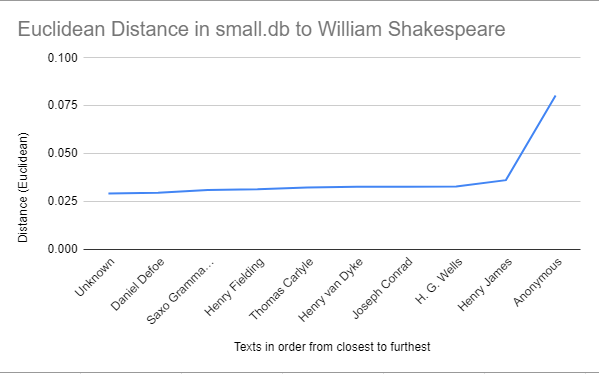
\includegraphics[width = 0.75\textwidth]{Graphs/Euclidean.PNG}

In the above graph is the nearest neighbors in small.db using the Euclidean distance from William Shakespeare's text, which matches the order of the example binary. The Euclidean distance is the metric that has the distances with the least average values, since in the algorithm to calculate, we have to computer the square root of the sum at the end of the calculation. While the Euclidean distance says that Saxo Grammaticus is the most likely author out of the small.db authors to be the one to write William Shakespeare's text, the other metrics don't agree.

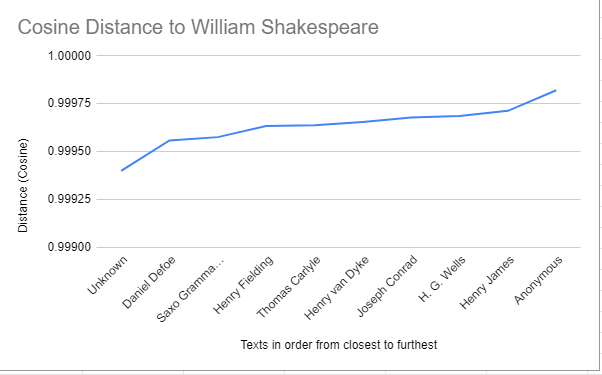
\includegraphics[width = 0.75\textwidth]{Graphs/Cosine.PNG}
\\ \\
The above graph shows the Cosine distance of the texts in small.db to William Shakespeare's text. The calculations essentially generate a larger sum based on the similarity of the texts and subtract that sum from 1. In the case for this calculation, the numbers are much higher than those of the Euclidean distance, and they also produce a different result. According to the Cosine distance calculation, the Unknown author is the most likely author to be the one to write Shakespeare's text.
\\ \\
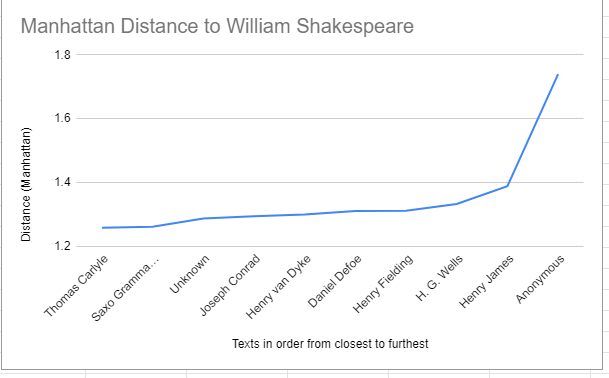
\includegraphics[width = 0.75\textwidth]{Graphs/Manhattan.PNG}
\\ \\
The above graph shows the Manhattan distance of the texts in small.db to Shakespeare's text once again. These calculations are even larger, since the calculation simply gets the sum of the difference between vectors. This metric claims that Thomas Carlyle is the most likely author of Shakespeare's text. All 3 of these metrics agree on which text is the most unlikely text, which is the anonymous text, but only Manhattan and Euclidean agree that the author is most likely either Thomas Carlyle or Saxo Gramaticus, since their values are extremely close in distance. Overall, all three of these distance calculations give different results and can be used in different ways to compute a variety of different ways to interpret distance. \\
\section{Texts and Priorty Queue}\label{ss:Texts}
Inside my program, the part that runs the longest is in the Text.c files because they have to potentially iterate over the large hash table for each word inside the given text. The potential O(n) lookup in a worst case scenario for the larger texts is what makes the program run for so long. In specific, the creation of the text is what takes the longest since it has to iterate over an entire text in order to add each word to the hash table. \\ \\
When creating the texts, we have to use our regular expressions to only accept viable words. I noticed that when I ran my program with a faulty regular expression, the computed distances were very off, but fixing my regular expression made the distances much closer and ordered the authors in the correct way. My program still has differences in the rounding when compared to the example binary, and since the regular expression that I used should be accepting all the viable words for this assignment, the difference in distance must be in my algorithm.
\\ \\
When implementing my Priority Queue, I did this aspect last since I was able to reuse my old pq.c ideas from assignment 6. Most of my original functions follow the same ideas and structure as my old priority queue, other than what I had to change to fit the different parameters for creating, enqueuing, and dequeuing. Following  Eugene's advice in section, I incorporated a local struct that I would use for enqueuing and dequeuing that contained the author and the corresponding distance. I did not use memory allocation for these since I was not creating an array for the author and distance, so I did not create a destructor for this struct. I ran into an issue with the priority queue near the end of this assignment, where when I would enqueue an author and distance, the previous authors would get overwritten since they all pointed to the same memory address and the value at that address would change with each loop. I had to duplicate the string and enqueue the duplicate in order to solve this problem, which also made me have to free all the remaining authors in the priority queue that I did not dequeue in order to avoid haveing memory leaks.
\\
\section{Other Comments}\label{ss:comments}
This program took a long time to compile in Valgrind, even for the small database, so I did not check this program with the large database through Valgrind, but I would assume that if the program is able to run without memory leaks in the smaller database, that it would not cause a problem checking for leaks in a larger database. I also tried to decrease the floating point round off errors using long doubles instead of doubles, but since the specified return values for the given functions are in doubles, I was not able to decrease the rounding error by a lot. While there is still a difference in the values for my program and the example binary executable, the results in terms of most likely authors is mostly the same. In my Makefile, I also compiled the program using -Ofast, because my program's run speed was very slow when trying to test, and using that compiler flag I was able to cut the run time down by a few seconds.
\end{document}
